\section{Updated Opacities}\label{sec:opac}
% Radiative opacity is fundamental to stellar structure, it determines how much
% incident radiation is absorbed or scattered. Moreover, when a media is in
% thermodynamic equilibrium with the radiation field, that is when the temperature
% of the media and that of the radiation field is the same, the opacity may be
% used via Kirchhoff's law to find the emissivity of a material
% \citep{Huebner2014}. Local Thermodynamic Equilibrium (LTE) is a common state to
% find within a star and therefore stellar models have long relied on opacities
% calculated in LTE.
OPAL high-temperature radiative opacity tables in particular are very widely
used by current generation isochrone grids \citep[e.g. Dartmouth, MIST, \&
StarEvol, ][]{Dotter2008,Choi2016,Amard2019}. However, there are two primary
issues with these tables, one, they are relativly old and therefore do not
incorperate the most up to date understanding of plasma modeling in their code
{\color{red} [CITATION]}, and two, they report rossland mean opacitieis to only
{\color{red} N} digits {\color{red} [WHICH IS AN ISSUE WHY?]}.

While the two issues given above should have relativly small affects, the
strong theoretical opacity dependence of the Jao Gap raises the potential for
these small effects to measurably shift the gap's location. In order to address
both the out of date plasma modeling and the low numeric presicion we update
DSEP to use high temperature opacity tables based on measurements from Los
Alamos national Labs T-1 group \citep[OPLIB,][]{Colgan2016}. The OPLIB tables
use the much more up-to-date ATOMIC plasma modeling code {\color{red}
[CITATION]} in addition to reporting rossland mean opacities to {\color{red} N}
digits of numeric presicion.

ATOMIC \citep{Magee2004} is a LTE and non-LTE opacity and plasma modeling code.
A major strength of ATOMIC when compared to the older plasma modeling programs
is its ability to vary its refinement level \citep{Fontes2016}.
{\color{red}[OTHER DIFFERENCES]} For a more detailed breakdown of how the most
up-to-date set of OPLIB tables are generated see \citep{Colgan2016}.

The most up to date OPLIB tables include monochromatic Rosseland mean opacities
--- composed from bound-bound, bound-free, free-free, and scattering opacities
--- for elements hydrogen through zinc over temperatures 0.5eV to 100 keV and
for mass densities from approximately $10^{-8}$ g cm$^{-3}$ up to approximately
$10^{4}$ g cm$^{-3}$ (though the exact mass density range varies as a function
of temperature). 

When comparing OPAL and OPLIB opacity tables (Figure \ref{fig:opacComp}) we
find OPLIB opacities are systematically lower than OPAL opacities for
temperature above $10^{6}$ K (Figure \ref{fig:opacComp}). These lower opacities
will result the temperature where radiation dominates energy transport lowering
{\color{red} [CITATION?]}. Consequently, the radiative layer in stellar models
evolved using OPLIB opacity tables will be {\color{red} [further?]} out from
the models center than it would be in models making use of OPAL tables.

\begin{figure}
	\centering
	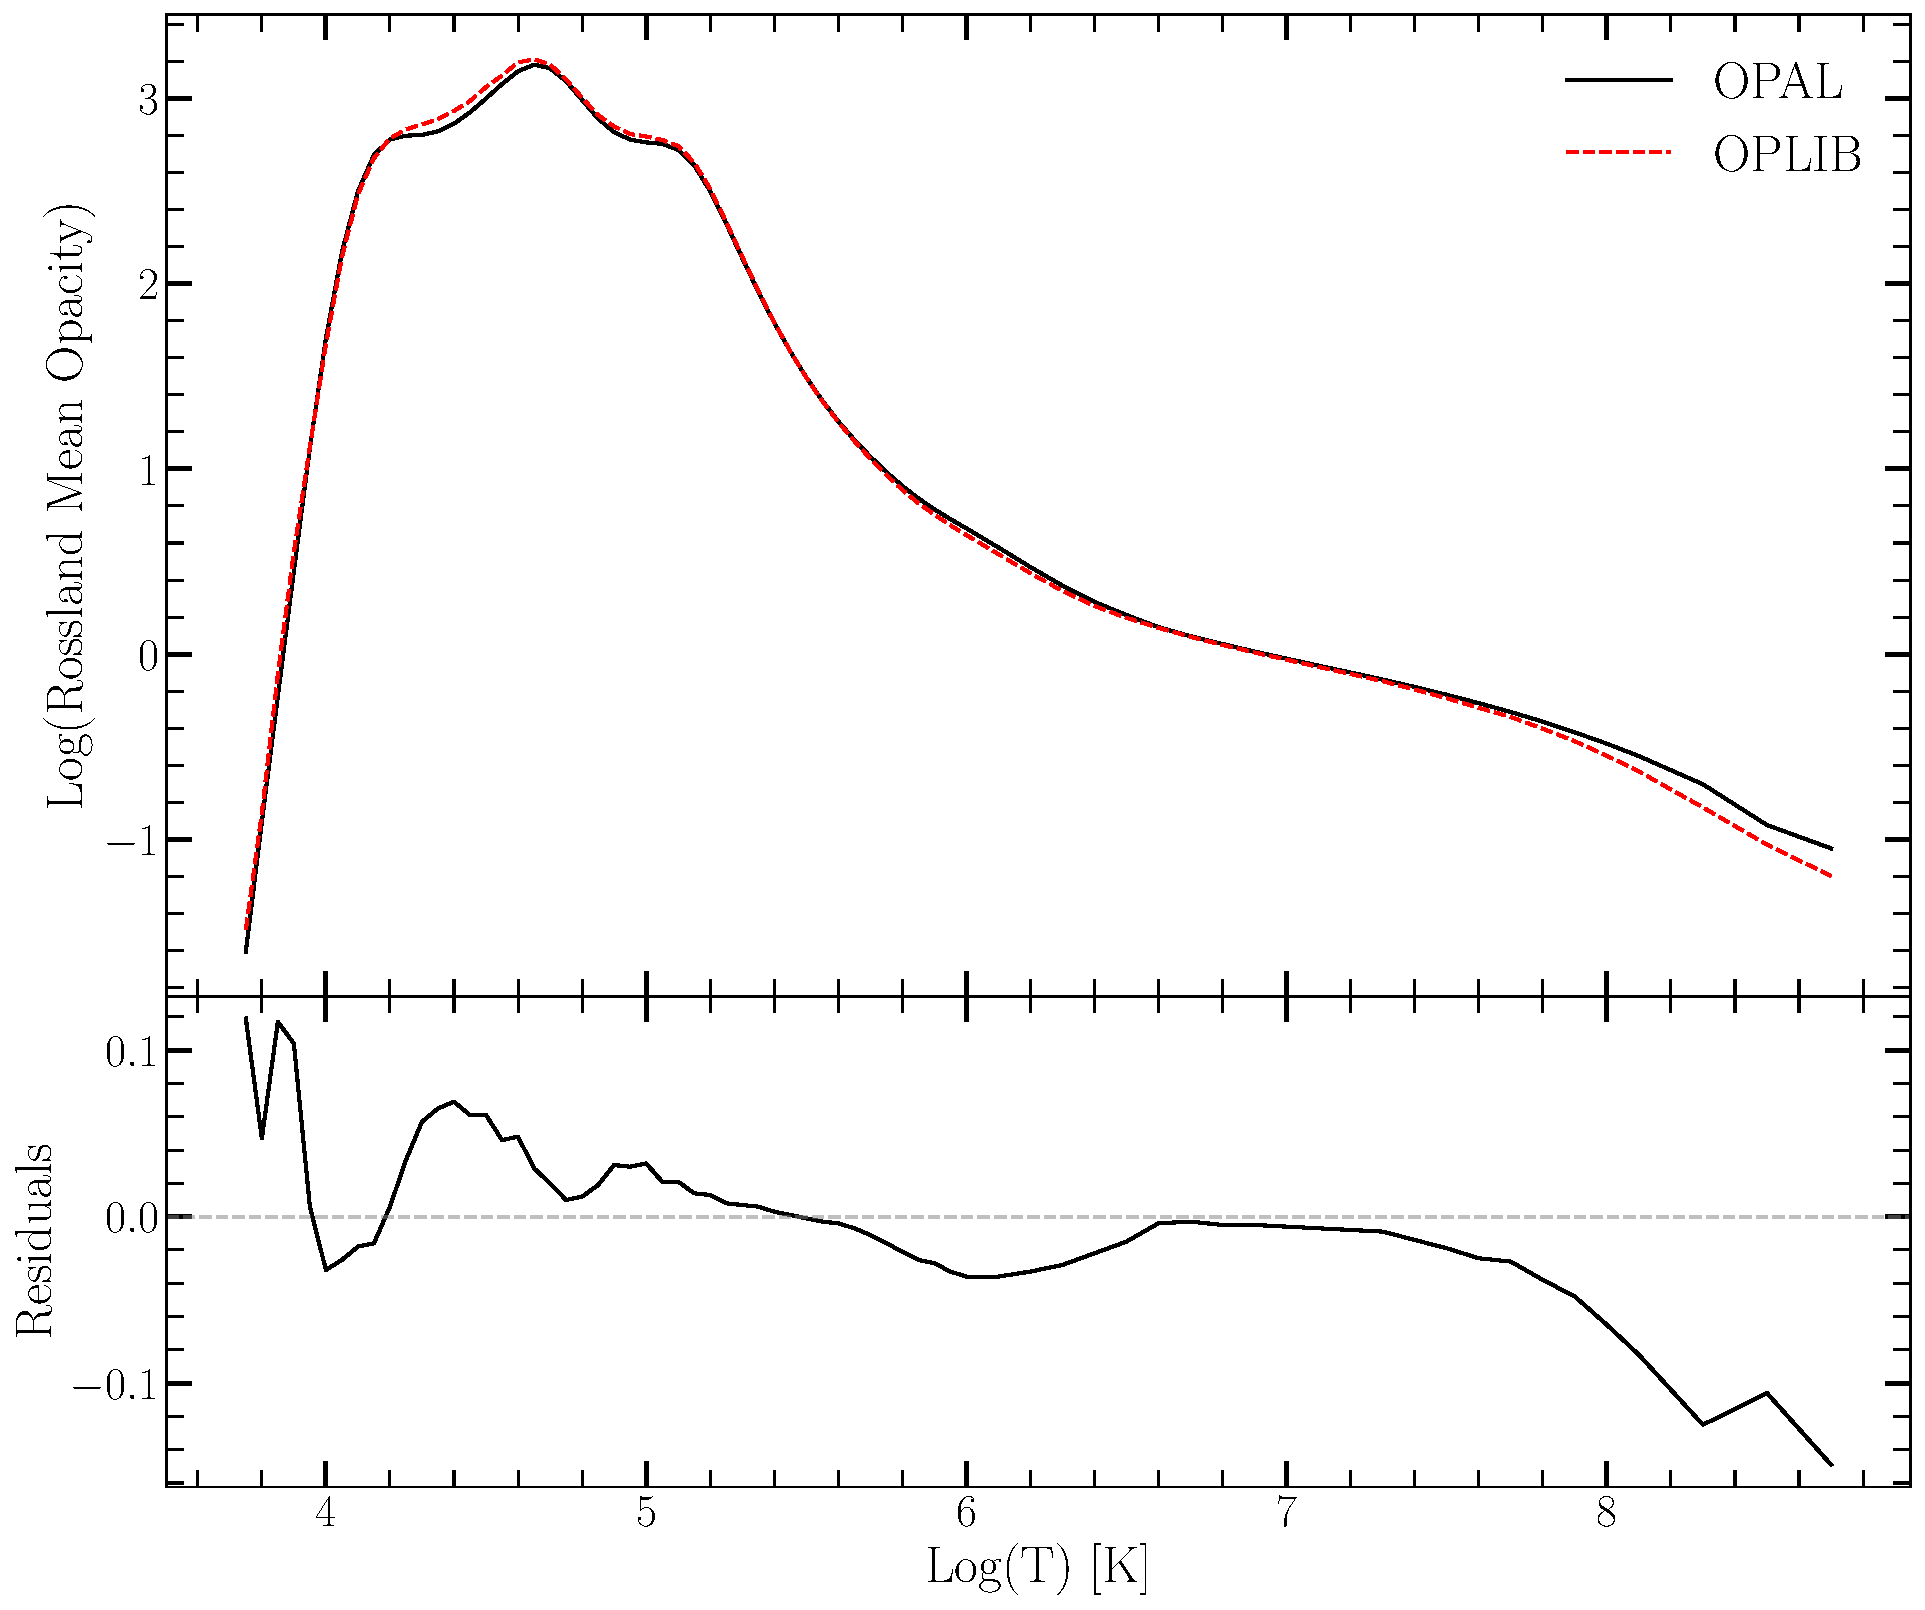
\includegraphics[width=0.45\textwidth]{src/figures/OpacityComparision.pdf}
	\caption{Rosseland mean opacity with the GS98 solar composition for both
	OPAL opacities and OPLIB opacities (top). Residuals between OPLIB opacities
	and OPAL opacities (bottom). These opacities are plotted at $\log _{10}(R)
	= -1.5$, $X=0.7$, and $Z=0.02$. Note how the OPLIB opacities are
	systematically lower than the OPAL opacities for temperatures above $10^6$
	K.}
	\label{fig:opacComp}
\end{figure}

\subsection{Table Querying and Conversion}
DSEP, along with most other stellar evolution programs, uses pre-computed
high-temperature opacity tables. Specifically, these tables list the
Rosseland-mean opacity, $\kappa_{R}$, along three dimensions: temperature, a
density proxy $R$, and composition. $R$ is defined as

\begin{align} \label{eqn:Req}
	R = \frac{\rho}{T_{6}^{3}}
\end{align}

Where $T_{6} = T\times10^{-6}$ and $\rho$ is the mass density. If $T$ and
$\rho$ are given in cgs then for much of the radius of a star $\log(R)\sim-1.5$
{\color{red}[CITATION]}.  $R$ is used, as opposed to simply tracking opacity
over mass density, because of its small dynamic range when compared to $\rho$ ($\rho\sim
10^{5}$ [g cm$^{-3}$] at the core of an RGB star all the way down to $\sim
10^{-8}$ [g cm$^{-3}$] within the envelope). 

OPLIB tables are queried from a web
interface\footnote{https://aphysics2.lanl.gov/apps/}. In order to generate many
tables easily and quickly we develope a web scraper built with Python's
\texttt{requests} module in addition to the 3rd party \texttt{mechanize} and
\texttt{BeautifulSoup} modules \citep{chandra2015python,
richardson2007beautiful} which can get tables with minimal intervention. This
web scraper submits a user requested chemical composition (composed of mass
fractions for elements from Hydrogen to Zinc) to the Los Alamos web form,
selects 0.0005 keV as the lower temperature bound and 60 keV as the upper
temperature bound, and finally requests opacity measurements for 100 densities,
ranging from $1.77827941\times 10 ^{-15}$ [g cm$^{-3}$] up to $1\times10^{7}$
[g cm$^{-3}$], at each temperature interval. These correspond to approximately
the same temperature and density range of opacities present in the OPAL opacity
tables.

OPLIB reports $\kappa_{R}$ as a function of mass density, temperature in keV,
and composition. Recall that DSEP accepts tables where opacity is given as a
function of temperature in Kelvin, $R$, and composition. The conversion from
temperature in keV to Kelvin is trivial
\begin{align}
	T_{K} = T_{keV} * 11604525.0061657
\end{align}
However, the conversion from mass density to $R$ is more involved. Because $R$ is
coupled with both mass density and temperature there there is no way to
directly convert tabulated values of opacity reported in the OPLIB tables to
their equivalents in $R$ space. Instead we must rotate the tables,
interpolating $\kappa_{R}(\rho,T_{eff}) \rightarrow \kappa_{R}(R,T_{eff})$. 

To preform this rotation we use the \texttt{interp2d} function within
\texttt{scipy}'s \texttt{interpolate} \citep{2020SciPy-NMeth} module to
construct a cubic bivariate B-spline \citep{Dierckx1981} interpolating function
$s$, with a smoothing factor of 0, representing the surface $\kappa_{R}(\rho,
T_{eff})$. For each $R^{i}$ and $T^{j}_{eff}$ which DSEP expects
high-temperature opacities to be reported for, we evaluate Equation
\ref{eqn:Req} to find $\rho^{ij} = \rho(T^{j}_{eff},R^{i})$.  Opacities in
$T_{eff}$, $R$ space are then inferred as $\kappa^{ij}_{R}(R^{i},T^{j}_{eff}) =
s(\rho^{ij}, T^{j}_{eff})$. 

As first-order validation of this interpolation scheme we can preform a similar
interpolation in the opposite direction, rotating the tables back to
$\kappa_{R}(\rho, T_{eff})$ and then comparing the initial, ``raw'', opacities
to those which have gone through the interpolations process. Figure
\ref{fig:fracdiff} shows the fractional difference between the raw opacities
and a set which have gone through this double interpolation. The red line
denotes $Log(R)=-1.5$ where models will tend to sit for much of their radius.
Along the $Log(R)=-1.5$ line the mean fractional difference is $\langle \delta
\rangle = 0.006$ with an uncertainty of $\sigma_{\langle\delta\rangle} =
0.009$. One point of note is that, because the initial rotation into $Log(R)$
space also reduces the domain of the opacity function interpolation-edge
effects which we avoid initially by extending the domain past what DSEP needs
cannot be avoided when interpolating back into $\rho$ space. {\color{red} [IS
THERE SOME MORE CLEAR VALIDATION WHICH I SHOULD PREFORM?]}

\begin{figure}
	\centering
	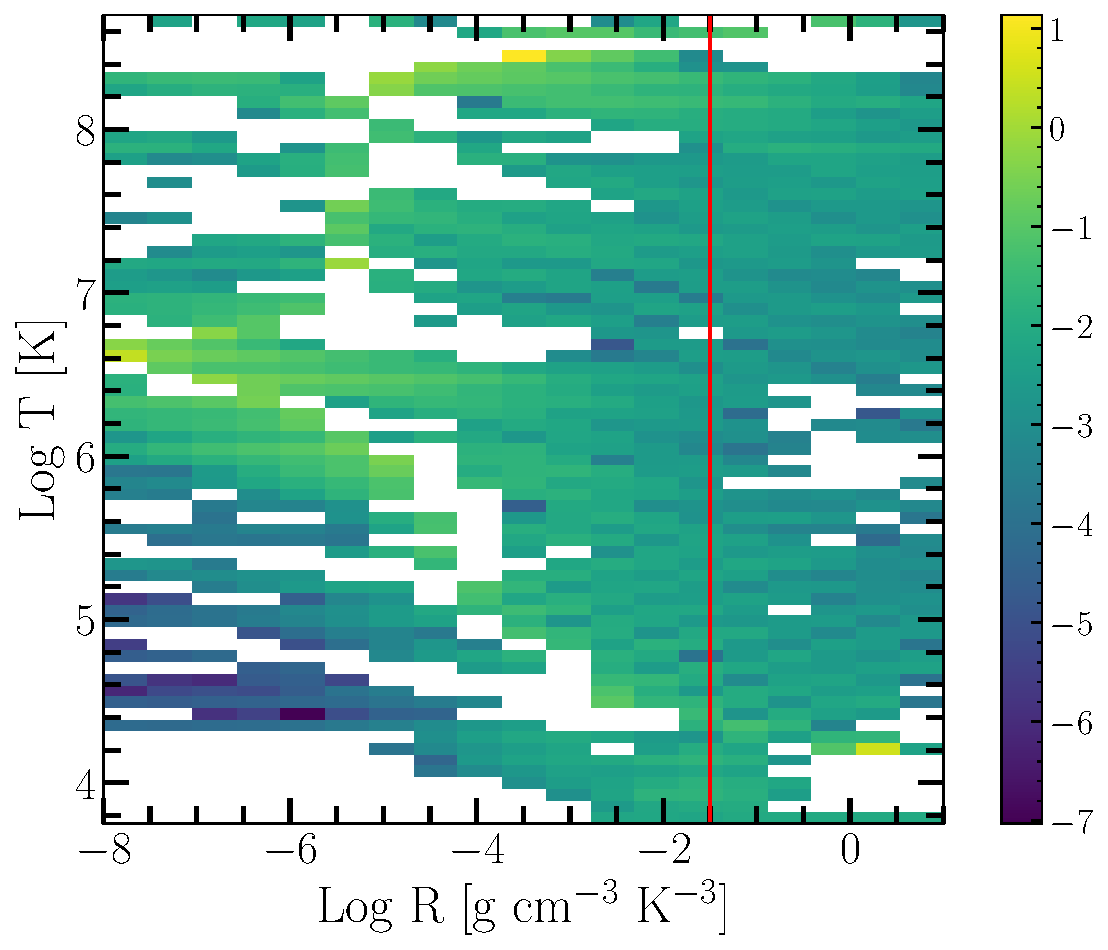
\includegraphics[width=0.45\textwidth]{src/figures/FractionalDifference.pdf}
	\caption{Log Fractional Difference between opacities in $\kappa_{R}(\rho,
	T_{eff})$ space directly queried from the OPLIB webform and those which
	have been interpolated into $Log(R)$ space and back. Note that, due to the
	temperature grid DSEP uses not aligning perfectly which the temperature
	grid OPLIB uses there may be edge effects where the interpolation is poorly
	constrained. The red line corresponds to $Log(R) = -1.5$ where much of a
	stellar model's radius exists.}
	\label{fig:fracdiff}
\end{figure}

